% Mirror: https://github.com/SIGma-UIUC/presentation-format
% --------------------------------------------------------------------
% This is a simple Beamer document that uses beamerthemesigma.sty
% Reading the comments should help you create a presentation even if
% you've never used Beamer before.
% --------------------------------------------------------------------

% Set our document class to Beamer
\documentclass[aspectratio=169]{beamer}
% \documentclass[aspectratio=169, handout]{beamer}
% Add handout option to ignore pauses

% From Jeff E
\usepackage{algo}
% Some more macros
\usepackage{sigmastyle}


% Set a title
\title{The Greatest Code of Them All}

% Set a subtitle if you desire
\subtitle{Reed-Solomon Codes}

% Whoever worked on the presentation:
\author{Anakin}

% Date looks ugly, so leave blank
\date{}

% An institute name, if you're so inclined
% \institute{University of Illinois Urbana-Champaign}

% Use the SIGma theme for this Beamer presentation
\usetheme{sigma}
% --------------------------------------------------------------------

% Begin document
\begin{document}

% Beamer calls each slide a "frame", defined within the environment:
% \begin{frame}
%   <frame content here>
% \end{frame}

% This frame is just the title.
\begin{frame}
\titlepage
\end{frame}

\section{Introduction}
\frame{\sectionpage}

\begin{frame}{Idea}
    \begin{itemize}
        \item \textcolor{sigma@alertred}{How many roots does a degree $d$ polynomial have?}\pause 
        \begin{itemize}
            \item Fundamental Theorem of Algebra say \textcolor{sigma@mainblue}{$\leq d$ roots}
        \end{itemize} \pause
        \item \textcolor{sigma@mainblue}{Idea:} Encode messages as evaluations of polynomials
        \item Few roots $\implies$ good distance
    \end{itemize}
\end{frame}

\begin{frame}{}
    \emph{Notation:}
    \begin{itemize}
        \item $\F_q = $ ``Integers mod $q$'' where $q$ is a prime power (Finite Field)
        \item $\F_q[x] = $ Polynomials with coefficients in $\F_q$
    \end{itemize}\pause
    \vspace{10pt}
    \begin{defn}[Reed-Solomon Codes \cite{rs}]
        Let $q \geq n \geq k$.
        Let $\alpha_1, \ldots, \alpha_n \in \F_q$ be distinct \emph{evaluation points}.
        The \emph{Reed-Solomon Code} of dimension $k$ with alphabet $\F_q$ and evaluation points $\vec{\alpha} = [\alpha_1, \ldots, \alpha_n]$ is
        \[
            \textsc{RS}_q(\vec{\alpha}, n, k) = \Set{ \bqty{f(\alpha_1), \ldots, f(\alpha_n)} | f \in \F_q[x],~ \deg(f) \leq k - 1}
        \]
    \end{defn}
\end{frame}

\begin{frame}{Encoding}
    \begin{defn}[Reed-Solomon Codes \cite{rs}]
        Let $q \geq n \geq k$.
        Let $\alpha_1, \ldots, \alpha_n \in \F_q$ be distinct \emph{evaluation points}.
        The \emph{Reed-Solomon Code} of dimension $k$ with alphabet $\F_q$ and evaluation points $\vec{\alpha} = [\alpha_1, \ldots, \alpha_n]$ is
        \[
            \textsc{RS}_q(\vec{\alpha}, n, k) = \Set{ \bqty{f(\alpha_1), \ldots, f(\alpha_n)} | f \in \F_q[x],~ \deg(f) \leq k - 1}
        \]
    \end{defn}\pause
    Say we want to encode a message $\vec{m} = [m_0, m_1, \ldots, m_{k - 1}]$, $m_i \in \F_q$ \pause
    
    Let $f_{\vec{m}}(x) \defeq  \Sum_{i = 0}^{k - 1} m_i x^i$ \pause
    \[
        \textsc{ENC}(m_0, \ldots, m_{k - 1}) = \bqty{f_{\vec{m}}(\alpha_1), \ldots, f_{\vec{m}}(\alpha_n)}
    \]
\end{frame}

\begin{frame}{Linearity}
    \begin{defn}[Reed-Solomon Codes \cite{rs}]
        $\textsc{RS}_q(\vec{\alpha}, n, k) = \Set{ \bqty{f(\alpha_1), \ldots, f(\alpha_n)} | f \in \F_q[x],~ \deg(f) \leq k - 1}$
    \end{defn}\pause
    \begin{itemize}
        \item $\textsc{RS}_q(\vec{\alpha}, n, k)$ is a \emph{linear} code
        \begin{itemize}
            \item Polynomials of degree $\leq k - 1$ in $\F_q[x]$ are a $k$-dimensional vector space
        \end{itemize}\pause
        \item If you recall from Hassam's meeting on linear codes, linear codes have generator matrices
    \end{itemize}
    \[
    G = \begin{bmatrix}
        1 & \alpha_1 & \alpha_1^2 & \cdots & \alpha_1^{k - 1} \\
        1 & \alpha_2 & \alpha_2^2 & \cdots & \alpha_2^{k - 1} \\
        \vdots & \vdots & \alpha_2^2 & \cdots & \vdots \\
        1 & \alpha_n & \alpha_n^2 & \cdots & \alpha_n^{k - 1} \\
    \end{bmatrix}
    \]
\end{frame}

\begin{frame}{Example}
    Let $q \geq n \geq k$ be $7 \geq 4 \geq 3$ respectively.
    Let $\vec{\alpha} = \bqty{\alpha_1, \ldots, \alpha_n} = [1, 2, 4, 6]$. \pause
    \[
        \textsc{ENC}(m_0, \ldots, m_{k - 1}) = \bqty{f_{\vec{m}}(\alpha_1), \ldots, f_{\vec{m}}(\alpha_n)}
    \]
    Lets encode $[m_0, m_1, m_2] = [1, 3, 5]$.
    \[
        f_{\vec{m}}(x) \defeq  \Sum_{i = 0}^{k - 1} m_i x^i = \textcolor{sigma@alertred}{???}
    \] % Spacing hacking going on here
    {\color{white}\[
        [f_{\vec{m}}(\alpha_1), f_{\vec{m}}(\alpha_2), f_{\vec{m}}(\alpha_3), f_{\vec{m}}(\alpha_4)] = [2, 6, 2, 3]
    \]}
    \textcolor{white}{How do we decode?}
\end{frame}

\begin{frame}{Example}
    Let $q \geq n \geq k$ be $7 \geq 4 \geq 3$ respectively.
    Let $\vec{\alpha} = \bqty{\alpha_1, \ldots, \alpha_n} = [1, 2, 4, 6]$.
    \[
        \textsc{ENC}(m_0, \ldots, m_{k - 1}) = \bqty{f_{\vec{m}}(\alpha_1), \ldots, f_{\vec{m}}(\alpha_n)}
    \]
    Lets encode $[m_0, m_1, m_2] = [1, 3, 5]$.
    \[
        f_{\vec{m}}(x) \defeq  \Sum_{i = 0}^{k - 1} m_i x^i = 1 + 3x + 5x^2 \in \F_7[x]
    \] \pause
    \[
        [f_{\vec{m}}(\alpha_1), f_{\vec{m}}(\alpha_2), f_{\vec{m}}(\alpha_3), f_{\vec{m}}(\alpha_4)] = [2, 6, 2, 3]
    \]\pause
    How do we \emph{decode}?
\end{frame}

\begin{frame}{The Original Decoding Algorithm}
    Say we want to recover $\vec{m}$ from $[f(\alpha_1), \ldots, f(\alpha_n)]$.
    Here is the original algorithm from Reed and Solomon's paper: \pause
    \begin{enumerate}
        \item $\deg(f) = k - 1$ so choose any $k$ of the evaluations $f(\alpha_i)$ \pause
        \item \emph{Interpolate} these points and find the polynomial $f_{\vec{m'}}(x) = \Sum_{i = 0}^{k - 1} m_i' x^i$ defined by these points \pause
        \item Do this for all $\binom{n}{k}$ choices of evaluations, do majority voting to pick out the right coefficients $m_i$
    \end{enumerate}
\end{frame}

\begin{frame}{Lagrange Interpolation}
    \begin{itemize}
        \item \emph{Note:} If two polynomials of degree $\leq k - 1$ agree on $k$ points, they must be the same polynomial\pause
        \item Let $f(x)$ be some polynomial of degree $\leq k - 1$, $\alpha_1, \ldots, \alpha_{k}$ distinct points in $\F_q$ \pause
    \end{itemize}
    \[
        L(x) \defeq \sum_{i = 1}^{k} f(\alpha_i) \pqty{\prod_{\substack{j = 1 \\ i \neq j}}^{k} \frac{x - \alpha_j}{\alpha_i - \alpha_j}} = \text{ the \emph{Lagrange Interpolating polynomial}}
    \]\pause
    \emph{Claim:} $L(x) = f(x)$ for all $x$.
\end{frame}

\begin{frame}{Lagrange Interpolation}
    Let $f(x)$ be some polynomial of degree $\leq k - 1$, $\alpha_1, \ldots, \alpha_{k}$ distinct points in $\F_q$
    \[
        L(x) \defeq \sum_{i = 1}^{k} f(\alpha_i) \pqty{\prod_{\substack{j = 1 \\ i \neq j}}^{k} \frac{x - \alpha_j}{\alpha_i - \alpha_j}} = \text{ the \emph{Lagrange Interpolating polynomial}}
    \]\pause
    \[
    \Prod_{\substack{j = 1 \\ i \neq j}}^{k} \frac{x - \alpha_j}{\alpha_i - \alpha_j} =     
    \begin{cases}\pause
        1 & \text{if } x = \alpha_i \\\pause
        0 & \text{if } x \neq \alpha_i\ (\text{so } x = \alpha_j\text{ for some } i \neq j)
    \end{cases}
    \]
    {\color{white}$\implies$ $L(x) = f(x)$ on $k$ points $\implies$ $L(x) = f(x)$ on all points}
\end{frame}

\begin{frame}{Lagrange Interpolation}
    Let $f(x)$ be some polynomial of degree $\leq k - 1$, $\alpha_1, \ldots, \alpha_{k}$ distinct points in $\F_q$
    \[
        L(x) \defeq \sum_{i = 1}^{k} f(\alpha_i) \pqty{\prod_{\substack{j = 1 \\ i \neq j}}^{k} \frac{x - \alpha_j}{\alpha_i - \alpha_j}} = \text{ the \emph{Lagrange Interpolating polynomial}}
    \]
    \[
    f(\alpha_i) \cdot \Prod_{\substack{j = 1 \\ i \neq j}}^{k} \frac{x - \alpha_j}{\alpha_i - \alpha_j} =     
    \begin{cases}\pause
        f(\alpha_i) & \text{if } x = \alpha_i \\\pause
        0 & \text{if } x \neq \alpha_i\ (\text{so } x = \alpha_j\text{ for some } i \neq j)
    \end{cases}
    \]
    {\color{white}$\implies$ $L(x) = f(x)$ on $k$ points $\implies$ $L(x) = f(x)$ on all points}
\end{frame}

\begin{frame}{Lagrange Interpolation}
    Let $f(x)$ be some polynomial of degree $\leq k - 1$, $\alpha_1, \ldots, \alpha_{k}$ distinct points in $\F_q$
    \[
        L(x) \defeq \sum_{i = 1}^{k} f(\alpha_i) \pqty{\prod_{\substack{j = 1 \\ i \neq j}}^{k} \frac{x - \alpha_j}{\alpha_i - \alpha_j}} = \text{ the \emph{Lagrange Interpolating polynomial}}
    \]
    \[
     \sum_{i = 1}^{k} f(\alpha_i) \pqty{\prod_{\substack{j = 1 \\ i \neq j}}^{k} \frac{x - \alpha_j}{\alpha_i - \alpha_j}} = \pause f(\alpha_i) \text{ if } x = \alpha_i \text{ for some } i \\\pause
    \]
    $\implies$ $L(x) = f(x)$ on $k$ points \pause $\implies$ $L(x) = f(x)$ on all points
\end{frame}

\begin{frame}{History}
    \begin{itemize}
        \item 1960: Reed and Solomon publish their original paper \cite{rs} \pause
        \item 1968/1969: Berlekamp and Massey improve on the decoding algorithm \cite{bm1, bm2} \pause
        \item 1986: Berlekamp and Welch design an even faster decoding algorithm \cite{bw} \pause
        \item 1996 and beyond: List Decoding methods become more prevalent 
    \end{itemize}
\end{frame}

\begin{frame}{Applications}
    QR Codes
    \begin{figure}
        \centering
        
\includegraphics[width=0.375\textwidth]{qart1.png}
    \end{figure}\pause
    CDs were the first mass produced item to use Reed-Solomon Codes (combined with techniques for burst errors from last meeting!)
\end{frame}

\begin{frame}
    \begin{figure}
        \centering
        
\includegraphics[width=0.5\textwidth]{ai.png}
    \end{figure}
\end{frame}

\begin{frame}{}
      \begin{center}
    {\color{sigma@mainblue} \LARGE Questions?}
  \end{center}
\end{frame}

\section{The Singleton Bound}
\frame{\sectionpage}

\begin{frame}
    \begin{thrm}[Singleton Bound \cite{sb}]
        If $C$ is is code over an alphabet $\Sigma$ of size $q$ encoding messages of length $k$ into codes of length $n$ with distance $d$, then $k \leq n - d + 1$
    \end{thrm}
    Recall $R = \frac{k}{n}$ is the \emph{rate} of $C$
    \begin{figure}
        \centering
        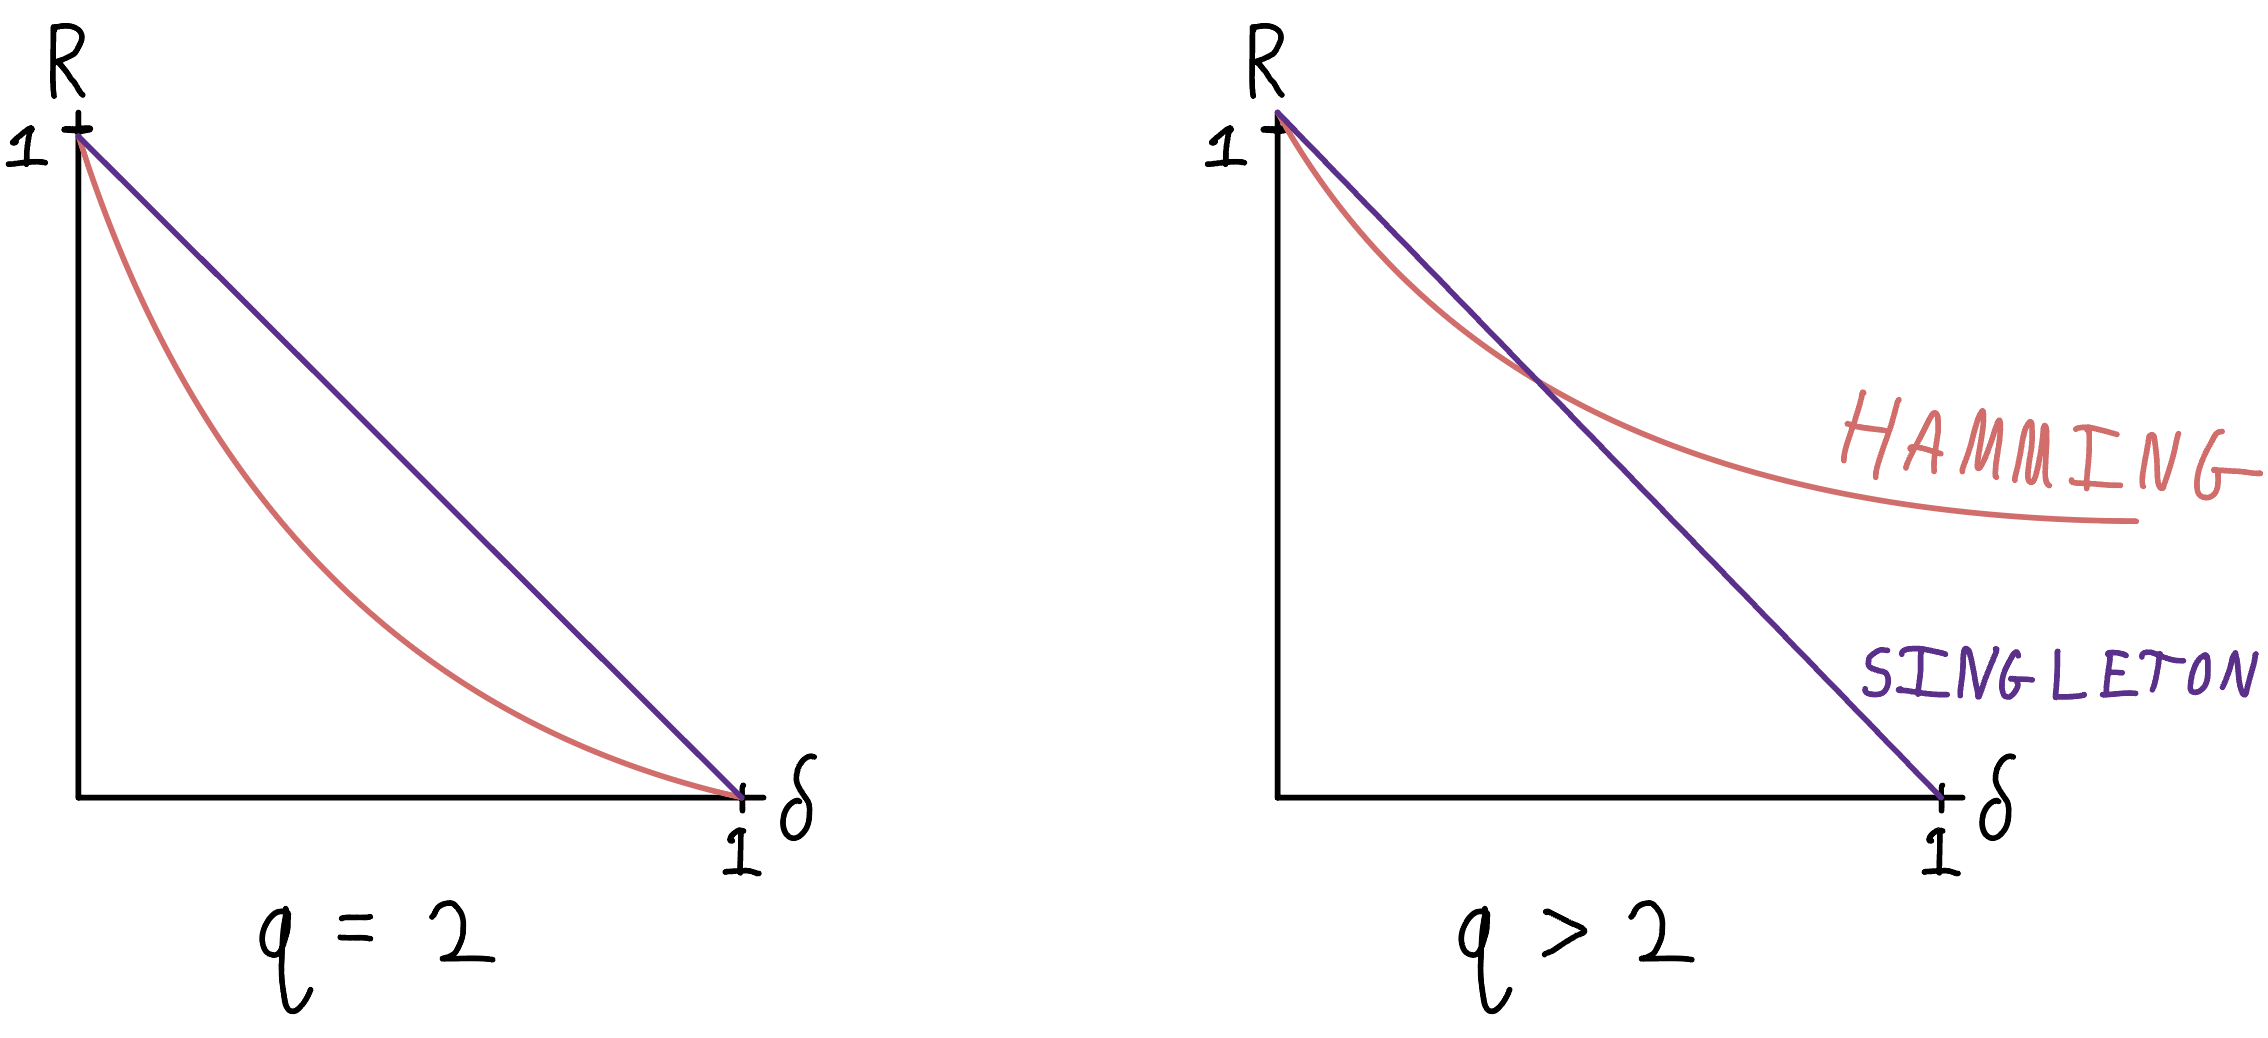
\includegraphics[width=\textwidth]{single.png}
    \end{figure}
\end{frame}

\begin{frame}{Proof of the Singleton Bound}
    \begin{thrm}[Singleton Bound \cite{sb}]
        If $C$ is is code over an alphabet $\Sigma$ of size $q$ encoding messages of length $k$ into codes of length $n$ with distance $d$, then $k \leq n - d + 1$
    \end{thrm}
    \begin{itemize}
        \item Let $c = (\overbrace{c_1, \ldots, c_{n - d + 1}}^{\phi(c)}, \overbrace{c_{n - d + 2}, \ldots, c_n}^\text{discard}) \in C$ \pause
        \item Let $\widetilde{C} = \Set{\phi(c) | c \in C} \subseteq \Sigma^{n - d + 1}$ 
        \item \emph{Claim:} $|C| = |\widetilde{C}|$
        \begin{itemize}
            \item If not, then $\phi(c) = \phi(c')$ for some $c \neq c' \in C$. \pause 
            Thus $\Delta(c, c') \leq d - 1$. \pause
            Contradicts fact that $C$ has distance $d$!
        \end{itemize} \pause
        \item Thus $|C| = |\widetilde{C}| \leq q^{n - d + 1}$
        \item $\implies k \defeq \log_q\abs{C} \leq n - d + 1$
    \end{itemize}
\end{frame}

\begin{frame}
    \begin{thrm}
        Reed-Solomon codes meet the Singleton Bound!
        The distance of $\textsc{RS}_q(\vec{\alpha} , k, n)$ is $d = n - k + 1$.
    \end{thrm} \pause
    \begin{itemize}
        \item The intuition for this is that the polynomials can have at most $k - 1$ zeroes so at most $k - 1$ of the $f(\alpha_i)$'s are $0$. \pause
        \item Distance $n - k - 1$ means we can correct $\leq \floor{\frac{n - k}{2}}$ errors
        \item We call Linear $(n, k, d)_q$ codes with distance $d = n - k + 1$ \emph{Maximum Distance Seperable} codes.\pause
    \end{itemize} 
    \begin{conj}[The MDS Conjecture \cite{mdsconj}]
        If $k \leq q$ then a linear MDS code has $n \leq q + 1$ unless $q = 2^h$ and $k = 3$ or $k = q - 1$ in which case $n \leq q + 2$.
    \end{conj}
\end{frame}

\begin{frame}{}
      \begin{center}
    {\color{sigma@mainblue} \LARGE Questions?}
  \end{center}
\end{frame}

\section{Berlekamp-Welch}
\frame{\sectionpage}

\begin{frame}{A Faster Decoding Algorithm}
    Given $(c_1, \ldots, c_n \in \textsc{RS}_q(\vec{\alpha} ,n, k)$ with $e \leq \floor{\frac{n - k}{2}}$ errors, we want to find $f \in \F_q[x]$ such that $\deg(f) \leq k$ and $f(\alpha_i) \neq c_i$ at most $e$ times.\pause
    
    Here is the idea behind the faster Berlekamp-Welch algorithm for decoding Reed-Solomon codes:
    \begin{itemize}
        \item Let $E(x) \defeq \Prod_{i\colon c_i \neq f(\alpha_i)}(x - \alpha_i)$ be the \emph{Error Locator Polynomial} \pause
        \item For all $1 \leq i \leq n$, we have that $c_i \cdot E(\alpha_i) = f(\alpha_i) \cdot E(\alpha_i)$
        \begin{itemize}
            \item If $c_i = f(\alpha_i)$ then this is obvious
            \item If $c_i \neq f(\alpha_i)$ then this is true because \pause $E(\alpha_i) = 0$
        \end{itemize} \pause
        \item The algorithm will find $E(x)$ and $Q(x) \defeq f(x) \cdot E(x)$
    \end{itemize}
\end{frame}

\begin{frame}{These Polynomials Exist}
    \begin{lem}
        Suppose there was some degree $\leq k - 1$ polynomial $f_{\vec{m}}(x) = \Sum_{i = 0}^{k - 1} m_i x^i$ such that $\Delta(m, c) \leq e$.
        Then there exist polynomials $E(x)$ \emph{monic} of degree $\leq e$ and $Q(x)$ of degree $\leq e + k - 1$ such that
        \[
            \text{for all } 1 \leq i \leq n,~c_i \cdot E(\alpha_i) = Q(\alpha_i)
        \]
    \end{lem}\pause
    \begin{itemize}
        \item $E(x) = \pqty{\Prod_{i\colon c_i \neq f(\alpha_i)}(x - \alpha_i)} * x^{e - \Delta(m, c)}$
        \item $Q(x) = E(x) \cdot f(x)$
    \end{itemize}
\end{frame}

\begin{frame}{System of Equations}
    Ok but how do we find $E(x)$ and $Q(x)$? \pause
    \begin{align*}
        E(x) \defeq \sum_{j = 0}^{e} e_j x^j && Q(x) \defeq \sum_{j = 0}^{e +k - 1} q_j x^j
    \end{align*}
    Since $c_i \cdot E(\alpha_i) = Q(\alpha_i)$, we have $c_i \cdot E(\alpha_i) - Q(\alpha_i) = 0$ for all $i$. \pause
    This gives $n$ linear equations, one for each $\alpha_i$:
    \[
        c_i \sum_{j = 0}^{e} e_j \alpha_i^j - \sum_{j = 0}^{e + k - 1} q_j \alpha_i^j = 0
    \]
    We have $n$ linear equations, and $2e + k$ variables.
    The \emph{Lemma} tells us that if there are not too many errors, some solution exists!
\end{frame}

\begin{frame}
    \begin{algo}
    \ul{\textsc{Berlekamp-Welch}($c = [c_1, \ldots, c_n]$):}
    \\  Find polynomials $E(x), Q(x) \in \F_q[x]$ such that\+
    \\      $E(x)$ is monic of degree $e$
    \\      $Q(x)$ is of degree $\leq e + k - 1$
    \\      For all $1 \leq i \leq n$:\+
    \\          $c_i \cdot E(\alpha_i) = Q(\alpha_i)$\-\-
    \\  If no solution: return \textsc{none}
    \\  $\widetilde{f}_{\vec{m}} \gets Q(x) / E(x)$
    \\  $\tilde{c} \gets \textsc{ENC}(m_0, \ldots, m_{k - 1})$
    \\  If $\Delta(\tilde{c}, c) > e$, return \textsc{none}
    \\  Return $\widetilde{f}_{\vec{m}}$
    \end{algo}\pause
    \begin{enumerate}
        \item Gaussian Elimination takes $O(n^3)$ time \pause
        \item Polynomial division will take $O(n^3)$ time \pause
        \item Computing $\tilde{c}$ will take $O(nk^2) \leq O(n^3)$ time \pause
        \item Computing $\Delta(\tilde{c}, c)$ takes $O(n)$ time
    \end{enumerate}
\end{frame}

\begin{frame}{}
      \begin{center}
    {\color{sigma@mainblue} \LARGE Questions?}
  \end{center}
\end{frame}

% Quotes are fun, find some to use!
\font\eightss=cmssq8
\font\eightssi=cmssqi8
\newcommand\quoteAuthorDate[3]{\begingroup
  \baselineskip 10pt
  \parfillskip 0pt
  \interlinepenalty 10000 % not needed in example
  \leftskip 0pt plus 40pc minus \parindent
  \let\rm=\eightss
  \let\sl=\eightssi
  \everypar{\sl}#1\par
  \nobreak\smallskip
  \noindent\rm--- #2\unskip\enspace(#3)\par
  \endgroup}
% If someone can figure out how to horizontally center this and make the text bigger that'd be cool
\begin{frame}
    \begin{center}
        \item \quoteAuthorDate{So long and thanks for all the fish!}{DOUGLAS ADAMS}{\color{sigma@mainblue} 1979}
    \end{center}
\end{frame}

% Remove this slide if you came up with all the material yourself
\nocite{intro}
\nocite{good_vids}
\begin{frame}[allowframebreaks]{Bibliography}
    \tiny
    \bibliography{refs}
    \bibliographystyle{alpha}
\end{frame}

\end{document}